\documentclass{article}
    \usepackage[francais]{babel}
    \usepackage[utf8]{inputenc}
    \usepackage[T1]{fontenc}
    \usepackage{lmodern}
    \usepackage{amsmath}
    \usepackage{amssymb}
    \usepackage{mathrsfs}
    \usepackage{tikz}
    \usepackage{graphicx}
    \usepackage{placeins}
    \usepackage{listings}
    \usepackage{cancel}
    \usepackage{hyperref}
    \usepackage{subcaption}
    \usepackage{xcolor}
    \colorlet{punct}{red!60!black}
    \definecolor{background}{HTML}{EEEEEE}
    \definecolor{delim}{RGB}{20,105,176}
    \colorlet{numb}{magenta!60!black}
    
    \newcommand{\deriv}{\mathrm{d}}
    \usepackage{array,multirow,makecell}
    \usepackage[top=2cm, bottom=3cm, left=2cm,right=2cm]{geometry}
    \usepackage{bbold}
    \newtheorem{problem}{Problem}
    \newtheorem{definition}{Definition}
    \newtheorem{conjecture}{Conjecture}
    \newtheorem{lemma}{Lemme}
    
    \usepackage{fancyhdr}
    \pagestyle{fancy}
    \fancyhead[L]{Marc-Antoine \bsc{Augé} - Team J5}
    \fancyhead[C]{Qualification - Abstract}
    \fancyhead[R]{Challenge ROADEF}
    \renewcommand{\headrulewidth}{1pt}
    \fancyfoot[C]{\thepage}
    
    \newcolumntype{C}[1]{>{\centering\arraybackslash }b{#1}}
    \setcounter{MaxMatrixCols}{20}
    \renewcommand{\footrulewidth}{1pt}
    
    \title{ROADEF / EURO Challenge 2018 \\
    - Qualification Submission (Team J5) -}
    \date{\today}
    \author{}
    
    \begin{document}
        \maketitle
\paragraph{Abstract}Our solution is simply a greedy-constructive algorithm, preceded by a thorough analysis of the problem in order to reduce the solution set. We modelized the solution set as a subset of :
\[ \mathcal{S}_0^N := ([|0, N|]\times\{0,1\}\times[|0, K - 1|]\times[|0, H - 1|]\times[|0, W - 1|])^N\]

Where $N$ is the number of items, $\{0, 1\}$ refers to the orientation of each item, $K$ is the number of bins available (100) and $H$ and $W$ are the dimensions of each bin ($6000\times 3210$). 


Each $s \in S_0$ is called a \textit{location} and is basically, an item, an orientation, a bin and a position for the lower-left corner on this bin. A solution is a vector of $S_0^N$. 
\begin{definition}[Notations]
    Let $s \in S_0$, we denote $(s_x, s_y)$ the coordinates of the lower-left corner, $(s_{xw}, s_{yh})$ the coordinates of the top-right corner.
\end{definition}

    \section{The Solution Set}
        
    $S_0^N$ is obviously too big : many $s_n \in S^N$ are not qualified and many could be easily improved.

    The problem was the following :
    
    \begin{problem}
    Let $0 \leq k  < N - 1$, let $(s^0, ..., s^k) \in S_0^k$ be a qualified solution, where items are cut in this order ($s^0$, ... , $s^k$). 
    
    Find $s_{k + 1} \in S_0$ such as $s(s_0, ..., s_{k + 1})$ is qualified and cannot be improved \textit{easily}.
    \end{problem}

    First of all, in order to explain how a solution can be \textit{easily improved} :

    \begin{conjecture}
        If $s^k$ and $s^k'\in S_0$ are two locations solutions of the problem 1, for the same item the same orientation, and :
        \begin{itemize}
            \item if $s^k_x == s^k'_x$ then the leftmost location is better
            \item if $s^k_{y} == s^k_{yw}$ then the lowest location is better
            \item else both locations could be good.
        \end{itemize}
    \end{conjecture}


        \subsection{The Green Star}
        First of all, we are ignoring the defects (\textit{cf} 1.3.)
        We introduced the \textit{Green Star} in order to restrict the solution set. The idea is to find locations which respect the guillotine cut constraint. An example is shown figure 1.a.
        
        \begin{definition}[The Green Star]
            The Green Star of $(s_0, ..., s_k)$ is defined by $ (x, y) \in [|0, W|]\times[|0, H|]$ such as there exists $i, j \leq k$ such that $x \leq s^i_{xw}$ and $y \leq s^j_{yh}$.
        \end{definition}
        
        \begin{conjecture}[The Green Star Condition]
            Every $s^{k + 1}$ must be out of the Green Star of $(s^0, ..., s^k)$ to be qualified.
        \end{conjecture}
        The Green Star can be greatly improved in order to give the list of locations (blue points) in $O(p)$ where $p$ is the number of points in the border of the Green Star (in practice, maximum 5).\\
        We used that method for the sprint phase. Unfortunately, some good locations are ignored : for example, the optimum for A1 with this method is 852.416. In fact, some blue points are unfeasable (the cutting tree is impossible) and thus locations on same $s_x$ are ignored.

        \subsection{The Red Monster}
    The Red Monster is the correction of the Green Star to keep optima locations. It is much more complex than the Green Star, since the Red Monster memorizes when each item must be cut, in order to remove unfeasable locations due to the cutting order.
    The figure 1.b shows the differences between both structures and how the Red Monster is able to accept the optima of A1, unlike the Green Star.

    \begin{figure}
        \centering
        \begin{subfigure}[b]{0.48\textwidth}
            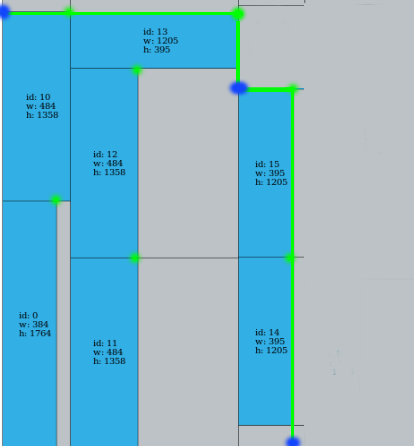
\includegraphics[height=7cm]{greenStart.png}
            \caption{The Green Star defines the few possible locations (blue points) which cannot be easily improved.}
            \label{fig:gull}
        \end{subfigure}
        ~ %add desired spacing between images, e. g. ~, \quad, \qquad, \hfill etc. 
          %(or a blank line to force the subfigure onto a new line)
        \begin{subfigure}[b]{0.48\textwidth}
            \centering
            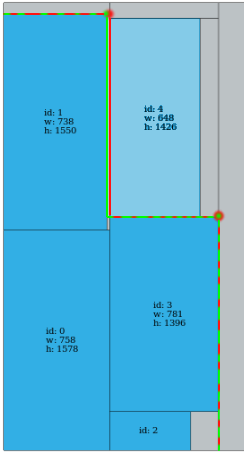
\includegraphics[height=7cm]{greenvsred.png}
            \caption{The Green Star VS the Red Monster : the Green Star tries a location more in the left that the Red Monster and therefore ignores the optima.}
            \label{fig:tiger}
        \end{subfigure}
        ~ %add desired spacing between images, e. g. ~, \quad, \qquad, \hfill etc. 
        %(or a blank line to force the subfigure onto a new line)
        \caption{Structures discovered and used}\label{fig:animals}
    \end{figure}

        \subsection{The Defects}
    The defects are roughly treated: for each possible location, if the location contains defects, we define a new Green Star with the defects contained in the bin in order to find the locations that are both free of defects and qualified. Yet, some optimizations are existing in practice.

        \subsection{The Tree Builder Algorithm}
    If the Red Monster seems to be able to find locations which are guillotine cut, there is no easy way to detect if the tree constraints are verified (depth, min-width...). 

    For each location, we try to build the tree for the complete bin : if it works, the location is feasible. It's a greedy recursive algorithm. In practice, only a little part of tree is necessary to check if a tree is always possible when a location is added.

    \section{Algorithm to Explore The Solutions}
        We implemented all this structures in C++ with many tricks in order to be able to quikly move along our solutions in both ways : adding new items or remove one. 

        The algorithm in our qualification submission is a branch-and-bound about that solution tree, where we decide the next location based on a heuristic score. This search algorithm could be improved to capitalize on the structures implemented. 

        
        Our results were obtained on a computer with \textbf{Intel(R) Core(TM) i7-3537U CPU @ 2.00GHz} (4 Cores) and 8Go Ram but our algorithm is mono-thread.

        
    \end{document}
    